\scanpage{2}
\margin{\uline{18.1.84}}
\mspage{1}
Conventions particulières et constructions relatives aux pos. rel. supersingulières. \unsure{Quatre} possibilités:

\margin{\uuline{Les 5 variantes de la \unsure{notion} de déploiement d'un syst. de pseudo-droites}}

1) On n'admet pas les p.r. supersing. parmi les sommets du graphe du départ, i.e. comme définissant des faces de $\mathcal X$.
On trouve une surface $\mathcal X_0$ dans laquelle les ``pos. rel. supersingulières'' correspondent \deleted{aux}\inserted{à un} ``\unsure{sommet|sommets} \unsure{supersingulier|supersinguliers}'' --- ce sont les seuls sommets qui sont d'ordre $4n$, au lieu d'être d'ordre $4$.

\margin{\uline{NB} Il n'y a pas de ``bouts libres'' (rouges) en un sommet supersingulier --- toute \deleted{droite} ps.dr. aboutissant (comme une face $\unsure{F_i|F}$ incidente à $s$) en $s$, se prolonge sur la face antipodique $\unsure{F'|F'_i}$, \unsure{à} $F$ en $s$)}
\figure{%
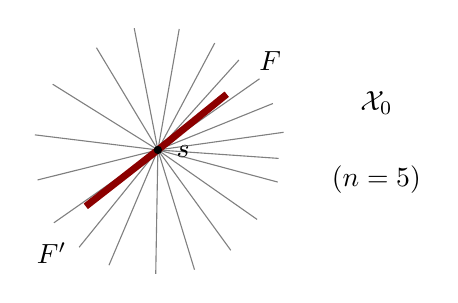
\begin{tikzpicture}[scale=.75]
\foreach \a/\r in {8/2.15,22/2.1,35/2.1,48/2.05,62/2.05,80/2.08,101/2.1,121/2.02,148/2.1,173/2.1,194/2.1,215/2.15,231/2.12,247/2.12,269/2.1,287/2.12,306/2.1,325/2.05,345/2.1,356/2.05}{\draw[gray] (0,0)--(\a:\r);}
\draw[red!55!black,line width=2.5pt] (39:1.5)--(0,0)--(218:1.55);
\fill (0,0) circle(2pt);\node[right] at (.15,-.03) {$s$};
\node at (1.9,1.5) {$F$};\node at (-1.8,-1.75) {$F'$};
\node at (3.7,.8) {$\mathcal X_0$};\node at (3.7,-.5) {$(n=5)$};
\end{tikzpicture}%
}

2) \deleted{Enfin}\inserted{On} admet les p.r. supersingulières comme \inserted{sommets} et les spécialisations directes (à partir d'une p.r. \uline{sous-stable}) vers celles-ci comme arêtes (correspondant, pour les p.r. sous-stables envisagées, à certains \uline{arcs de spécialisations} exceptionnels.
Finalement, il y a intérêt à les choisir aussi courts que possible (alors qu'au début je les choisissais aussi longs que possible), savoir de longueur combinatoire $1$, et placés à égale distance entre les arcs de transition (ou plutôt, de générisation) les plus proches). Ainsi, autour de la face supersingulière $F_i$ correspondant à une p.r. de générisation donnée, vont se raccorder (\deleted{\unsure{2n}}\inserted{le long de} $2(n-1)$ arcs de longueur combinatoire $1$ alors que) les $2(n-1)$ faces correspondant aux \unsure{\deleted{des}\inserted{positions}} relatives sous-stables proches, sans compter les \deleted{positions relatives}\inserted{(faces de) \unsure{biangles}}, stables proches, qui sont \deleted{\unsure{pris}} comprises \deleted{entre}\inserted{chacune entre} deux faces sous-stables avoisinantes, et touchant $F$ en \uline{un} sommet incident commun. Le nombre $2(n-1)$ est d'ailleurs correct, seulement dans le cas stable, dans le cas général c'est $2n_i$, où $n_i$ est le nb de sommets sur $D_i\unsure{\in|\subset}\Sigma_i$. Sur la surface $\mathcal X_1$ obtenue, tous les

\figure{%
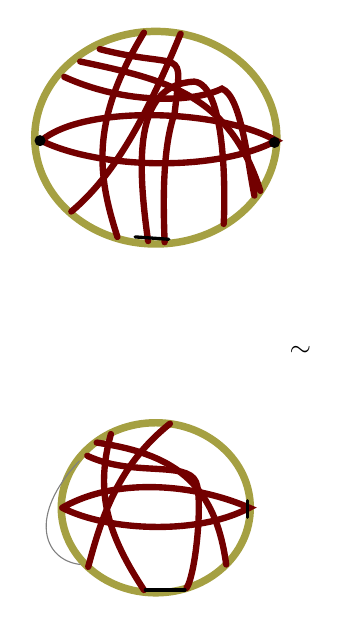
\begin{tikzpicture}[x=.75cm,y=.75cm,line cap=round]
\begin{scope}[yshift=4.7cm]
\draw[yellow!60!black,line width=2.7pt] (0,0) ellipse(2.05 and 1.8);
\draw[red!45!black,line width=2.3pt] (-1.94,-.05)..controls(-1.2,.57)and(1.1,.48)..(2.04,-.05)..controls(1,-.6)and(-1,-.52)..(-1.94,-.05);
\draw[red!45!black,line width=2.3pt] (-.2,1.78)..controls(-1.1,.3)and(-1.0,-.6)..(-.65,-1.68) (.42,1.76)..controls(-.1,.5)and(-.65,-.6)..(-1.43,-1.25);
\draw[red!45!black,line width=2.3pt] (-1.28,1.29)..controls(.2,.98)and(1.25,.72)..(1.77,-.9) (-1.55,1.03)..controls(-.5,.55)and(.66,.6)..(1.12,.83)..controls(1.45,.7)and(1.55,-.4)..(1.67,-.98);
\draw[red!45!black,line width=2.3pt] (-.95,1.5)..controls(.5,1.13)and(.45,1.6)..(.32,.42)..controls(.12,-.15)and(.12,-1.0)..(.15,-1.77) (-.13,-1.75)..controls(-.35,-.2)and(-.3,.9)..(.65,.95)..controls(1.18,.9)and(1.18,-.9)..(1.15,-1.46);
\draw[very thick] (-.35,-1.68)--(.22,-1.72);
\fill(-1.96,-.05)circle(2pt);\fill(2.01,-.08)circle(2pt);
\end{scope}
\node at (2.45,2.65) {$\unsure{\sim}$};
\begin{scope}[scale=.8]
\draw[yellow!60!black,line width=2.7pt] (0,0) ellipse(2 and 1.8);
\draw[red!45!black,line width=2.3pt] (-1.98,0)..controls(-.8,.68)and(.9,.48)..(1.98,0)..controls(.9,-.58)and(-1,-.5)..(-1.98,0);
\draw[red!45!black,line width=2.3pt] (-.95,1.56)..controls(-1.3,.3)and(-1,-.6)..(-.25,-1.74) (.3,1.78)..controls(-.8,.9)and(-1.15,-.2)..(-1.43,-1.25);
\draw[red!45!black,line width=2.3pt] (-1.45,1.1)..controls(-.5,.65)and(.65,1.0)..(.85,.55)..controls(1,.2)and(.85,-1.4)..(.65,-1.7);
\draw[red!45!black,line width=2.3pt] (-1.25,1.38)..controls(.3,1.15)and(1.25,.6)..(1.49,-1.2);
\draw[gray] (-1.62,.99)..controls(-2.7,-.15)and(-2.4,-1.1)..(-1.6,-1.2);
\draw[very thick] (-.22,-1.74)--(.62,-1.74);\draw[very thick](1.94,.15)--(1.94,-.2);
\end{scope}
\end{tikzpicture}%
}
\figure{%
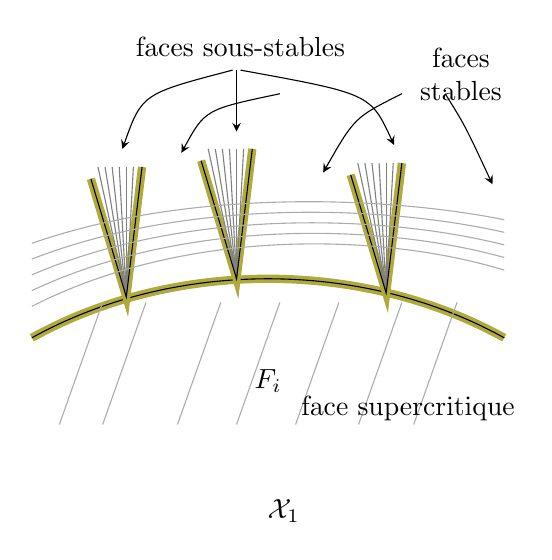
\begin{tikzpicture}[x=1cm,y=1cm,>=stealth]
\draw[yellow!65!black,line width=3pt] (-3,0)..controls(-1.2,1)and(1.2,1)..(3,0);
\draw[black] (-3,0)..controls(-1.2,1)and(1.2,1)..(3,0);
\foreach \x/\y in {-1.8/.52,-.4/.75,1.5/.57}{
\draw[yellow!65!black,line width=3pt] (\x-.45,\y+1.5)--(\x,\y)--(\x+.2,\y+1.65);
\foreach \d in {-.36,-.27,-.18,-.09,0,.09}{\draw[gray,thin] (\x,\y)--(\x+\d,\y+1.65);}
\draw (\x-.45,\y+1.5)--(\x,\y)--(\x+.2,\y+1.65);}
\foreach \j in {1,2,3,4,5}{\draw[gray!65,thin] (-3,.2+\j*.2)..controls(-1,1.3+\j*.12)and(1.5,1.2+\j*.12)..(3,.7+\j*.16);}
\foreach \x in {-2.1,-1.55,-.6,.15,.9,1.7,2.4}{\draw[gray!65,thin] (\x,.45)--(\x-.55,-1.1);}
\node at (0,-.55) {$F_i$};\node[right] at (.3,-.9) {face supercritique};
\node at (-.35,3.7) {faces sous-stables};
\draw[->] (-.4,3.4)--(-.4,2.62);\draw[->](-.45,3.4)..controls(-1.6,3.1)..(-1.85,2.4);\draw[->](-.35,3.4)..controls(1.3,3.1)..(1.6,2.45);
\node[align=center] at (2.45,3.35) {faces\\stables};
\draw[->] (2.25,3.1)..controls(2.5,2.7)..(2.85,1.95);
\draw[->] (1.7,3.1)..controls(1.1,2.8)..(.7,2.1);
\draw[->] (.15,3.1)..controls(-.8,2.9)..(-1.1,2.35);
\node at (.2,-2.2) {$\mathcal X_1$};
\end{tikzpicture}%
}
\margin{1}
